% ch11 Electron–lattice interactions (书页 169–188 / 分册p001–p020)
% 第11章 Electron–lattice interactions
\chapter{电子–晶格相互作用}

迄今为止，我们一直聚焦于电子问题，把离子当作固定在其平衡位置 $\mathbf{R}_i^0$ 处。在电子气的语境下，我们对离子采取了甚至更为简单的看法，即它们只提供一个均匀的补偿性正电荷背景。为了能够描述固体中观测到的各类物理，我们必须在处理离子运动时引入一些真实性。电子自由度与离子运动的耦合就是电子–声子问题。固体中的声子（phonon）源于离子的集体运动。这种运动是量子化的，并且是如下三类现象的根本成因：(1) 极化子（polaron）的形成；(2) 超导电性中电子间的吸引作用；(3) 金属中电阻率对温度的依赖。本章中，我们集中讨论电子–声子问题的一般表述，随后将其应用于金属的低温电阻率。

\section{谐振链}

我们从对一个由谐振弹簧相连的 $N$ 个原子构成的一维链的简要回顾（文献 [M1981]）开始。令 $x_i$ 表示每个振子偏离其平衡位置的位移，$\omega$ 为每根弹簧的振荡频率，$M$ 为每个原子的质量。此谐振链的总哈密顿量为
\begin{equation*}
H=\sum_i\frac{P_i^2}{2M}+\frac{M\omega^2}{2}\sum_i(x_i-x_{i+1})^2.\tag{11.1}
\end{equation*}
我们对动量作傅里叶变换
\begin{equation*}
P_n=\frac{1}{\sqrt{N}}\sum_k\mathrm{e}^{\mathrm{i}kna}P_k\tag{11.2}
\end{equation*}
并对位移算符作傅里叶变换
\begin{equation*}
x_n=\frac{1}{\sqrt{N}}\sum_k\mathrm{e}^{\mathrm{i}kna}x_k,\tag{11.3}
\end{equation*}
从而将此哈密顿量对角化，其中 $a$ 是晶格常数。注意到
\begin{equation*}
\sum_n P_n^2=\sum_k P_kP_{-k}\tag{11.4}
\end{equation*}
以及
\begin{equation*}
\sum_n x_nx_{n+m}=\sum_k x_kx_{-k}\mathrm{e}^{-\mathrm{i}kma},\tag{11.5}
\end{equation*}
我们便可把哈密顿量改写到 $k$ 空间：
\begin{equation*}
H=\frac{1}{2M}\sum_k P_kP_{-k}+\frac{M}{2}\sum_k\omega_k^2x_kx_{-k},\tag{11.6}
\end{equation*}
其中 $\omega_k^2=2\omega^2(1-\cos ka)=4\omega^2\sin^2 ka/2$。因此，激发 $k=0$ 模式不耗费能量。这是声学声子（acoustic phonon）的一个标志性特征。$k=0$ 模式对应于离子的整体平移。由平移不变性，这样的变换不可能改变能量。这类不需要能量的长波长玻色型激发称为戈德斯通模（Goldstone mode）（文献 [G1963]），第1章中已首次讨论过。在磁性系统（例如铁磁体与反铁磁体）中，也存在类似的长波长激发，它们在 $k=0$ 处不耗费能量。这类激发称为自旋波或磁振子（magnon），构成磁性系统中的低能激发，因而（举例来说）决定磁性系统对比热的贡献。

让我们定义新算符
\begin{equation*}
\tilde{Q}_k=x_k\left(\frac{M\omega_k}{2\hbar}\right)^{1/2}\tag{11.7}
\end{equation*}
与
\begin{equation*}
\tilde{P}_k=\frac{P_k}{(2M\omega_k\hbar)^{1/2}},\tag{11.8}
\end{equation*}
借助它们可以将 $H$ 改写成富有启发性的形式
\begin{equation*}
H=\sum_k\hbar\omega_k[\tilde{P}_k\tilde{P}_{-k}+\tilde{Q}_k\tilde{Q}_{-k}].\tag{11.9}
\end{equation*}
一旦定义了产生算符
\begin{equation*}
b_k^{\dagger}=(\tilde{Q}_{-k}-\mathrm{i}\tilde{P}_{-k})\tag{11.10}
\end{equation*}
与湮灭算符
\begin{equation*}
b_k=(\tilde{Q}_k+\mathrm{i}\tilde{P}_k)\tag{11.11}
\end{equation*}
便可对 $H$ 作因式分解。$b_k$ 与 $b_k^{\dagger}$ 所服从的对易关系
\begin{equation*}
[b_k^{\dagger},b_{k'}]=-\delta_{kk'},\tag{11.12}
\end{equation*}
可由对易子
\begin{equation*}
[\tilde{P}_k,\tilde{Q}_{-k'}]=-\frac{\mathrm{i}}{2}\delta_{kk'}.\tag{11.13}
\end{equation*}
得到。因式分解后的哈密顿量具有我们熟悉的振子形式
\begin{equation*}
H=\sum_k\hbar\omega_k\left(b_k^{\dagger}b_k+\frac{1}{2}\right),\tag{11.14}
\end{equation*}
这表明系统是玻色子的集合。$b_k$ 的时间依赖
\begin{equation*}
b_k(t)=b_k(t=0)\mathrm{e}^{-\mathrm{i}\omega_k t},\tag{11.15}
\end{equation*}
通过求解海森堡运动方程
\begin{equation*}
-\mathrm{i}\hbar\dot{b}_k=[H,b_k]=-\hbar\omega_k b_k.\tag{11.16}
\end{equation*}
得到。算符 $b_k^{\dagger}(t)$ 在时刻 $t$ 产生一个频率为 $\omega_k$ 的集体晶格畸变。该畸变的空间图样由式 (11.10) 与式 (11.11) 解出 $x_k$
\begin{align*}
x_k(t)&=\frac{1}{2}\left(\frac{2\hbar}{M\omega_k}\right)^{1/2}\bigl(b_k(t)+b_{-k}^{\dagger}(t)\bigr)\\
&=\left(\frac{\hbar}{2M\omega_k}\right)^{1/2}\bigl(b_k\mathrm{e}^{-\mathrm{i}\omega_k t}+b_{-k}^{\dagger}\mathrm{e}^{\mathrm{i}\omega_k t}\bigr),\tag{11.17}
\end{align*}
再作傅里叶变换
\begin{equation*}
x_{\ell}(t)=\sum_k\left(\frac{\hbar}{2MN\omega_k}\right)^{1/2}\bigl(b_k\mathrm{e}^{-\mathrm{i}\omega_k t}+b_{-k}^{\dagger}\mathrm{e}^{\mathrm{i}\omega_k t}\bigr)\mathrm{e}^{\mathrm{i}k\ell a}.\tag{11.18}
\end{equation*}
而得到。$x_{\ell}(t)$ 的这个表达式告诉我们时刻 $t$ 在格点 $\ell$ 上晶格振动的振幅。对 $k$ 的求和限制在第一布里渊区内。

\section{声学声子}

为了与固体建立更具体的联系，我们考虑离子之间一般的成对相互作用势：
\begin{equation*}
V_{\mathrm{ion}}=\sum_{i<j}V(\mathbf{R}_i-\mathbf{R}_j).\tag{11.19}
\end{equation*}
离子的平衡位置 $\{\mathbf{R}_i^0\}$ 由每个离子所受净力为零的条件确定：
\begin{equation*}
\mathbf{F}_j=\sum_i\nabla V\bigl(\mathbf{R}_i^0-\mathbf{R}_j^0\bigr)=0.\tag{11.20}
\end{equation*}
于是，我们把每个离子的实际位置
\begin{equation*}
\mathbf{R}_i=\mathbf{R}_i^0+\mathbf{Q}_i,\tag{11.21}
\end{equation*}
表示为围绕平衡位置的展开。这里 $\{\mathbf{Q}_i\}$ 扮演线性链中 $\{x_i\}$ 的角色，因为它们表示每个离子偏离其原位的位移。每个离子在原位所受的力为零，这保证了离子势的泰勒展开
\begin{equation*}
V_{\mathrm{ion}}=\sum_{i<j}V\bigl(\mathbf{R}_i^0-\mathbf{R}_j^0\bigr)+\frac{1}{2}\sum_{i<j}(\mathbf{Q}_i-\mathbf{Q}_j)_{\mu}(\mathbf{Q}_i-\mathbf{Q}_j)_{\nu}F_{\mu\nu},\tag{11.22}
\end{equation*}
其中
\begin{equation*}
F_{\mu\nu}=\frac{\partial^2}{\partial R_{\mu}\partial R_{\nu}}V\bigl(\mathbf{R}_i^0-\mathbf{R}_j^0\bigr),\tag{11.23}
\end{equation*}
在围绕极小点的涨落的最低阶上是谐和的，式中重复指标求和。

与在一维链中一样，我们通过定义集体坐标
\begin{equation*}
\mathbf{Q}_i(t)=\sum_{\mathbf{k},\lambda}\left(\frac{\hbar}{2MN\omega_{\mathbf{k},\lambda}}\right)^{1/2}\bigl(b_{\mathbf{k},\lambda}\lambda_{\mathbf{k}}\mathrm{e}^{-\mathrm{i}\omega_{\mathbf{k},\lambda}t}+b_{-\mathbf{k},\lambda}^{\dagger}\lambda_{\mathbf{k}}^{*}\mathrm{e}^{\mathrm{i}\omega_{\mathbf{k},\lambda}t}\bigr)\mathrm{e}^{\mathrm{i}\mathbf{k}\cdot\mathbf{R}_i^0},
\end{equation*}
来将此相互作用对角化，其中 $\lambda_{\mathbf{k}}$ 是单位长度的极化矢量（polarization vector），依赖于声子的传播方向。对纵向声子，$\lambda_{\mathbf{k}}$ 平行于 $\mathbf{k}$；而对横向声子，$\lambda_{\mathbf{k}}$ 垂直于 $\mathbf{k}$。因为 $\mathbf{Q}_i$ 是厄米的，我们取极化矢量为纯实数。利用 $\mathbf{Q}_i(t)$ 的这一定义，我们把离子势
\begin{equation*}
V_{\mathrm{ion}}=\sum_{i<j}V\bigl(\mathbf{R}_i^0-\mathbf{R}_j^0\bigr)+\frac{M}{2}\sum_{\mathbf{k},\lambda}\omega_{\mathbf{k},\lambda}^2\mathbf{Q}_{\mathbf{k},\lambda}\mathbf{Q}_{-\mathbf{k},\lambda},\tag{11.24}
\end{equation*}
用声子或谐振模式 $\mathbf{Q}_{\mathbf{k},\lambda}$ 改写。对声学声子，$\mathbf{Q}_{\mathbf{k},\lambda}$ 描述邻近离子沿同一方向运动的畸变。这些对应于晶体的长波长模式。我们将只关注这类畸变。声子模式的共轭动量定义为（例如）在格点表象中计算 $\mathbf{P}_i=M\dot{\mathbf{Q}}_i$。$\mathbf{P}_i$ 与 $\mathbf{Q}_i$ 服从式 (11.13) 的正则对易关系。

\section{电子–声子相互作用}

在我们的普遍多体哈密顿量中，每个离子与电子之间的相互作用形如
\begin{equation*}
\begin{aligned}
V_{\mathrm{ei}}&=\sum_j V_{\mathrm{ei}}(\mathbf{r}_j)\\
&=\sum_{i,j}V_{\mathrm{ei}}(\mathbf{r}_j-\mathbf{R}_i).
\end{aligned}\tag{11.25}
\end{equation*}
为与上一节引入的声子展开衔接，我们把离子坐标写成对原位的偏离 $\mathbf{R}_i=\mathbf{R}_i^0+\mathbf{Q}_i$，并将电子–离子势在 $\mathbf{R}_i^0$ 附近作泰勒级数展开。准确到一阶，我们有
\begin{equation*}
V_{\mathrm{ei}}=\sum_{i,j}V_{\mathrm{ei}}\bigl(\mathbf{r}_j-\mathbf{R}_i^0\bigr)-\sum_{i,j}\mathbf{Q}_i\cdot\nabla_j V_{\mathrm{ei}}\bigl(\mathbf{r}_j-\mathbf{R}_i^0\bigr)+O(Q^2)+\cdots.\tag{11.26}
\end{equation*}
第一项定义了传导电子所见的周期势，因而关于电子与晶格畸变的耦合不包含任何新信息。这些信息包含在第二项中。为简化这一项，我们引入电子–离子势的傅里叶变换
\begin{equation*}
V_{\mathrm{ei}}(\mathbf{r})=\frac{1}{N}\sum_{\mathbf{k}}V_{\mathrm{ei}}(\mathbf{k})\mathrm{e}^{\mathrm{i}\mathbf{k}\cdot\mathbf{r}}.\tag{11.27}
\end{equation*}
有了这个定义，我们把电子–离子势写成
\begin{equation*}
V_{\mathrm{ei}}=V_0-\frac{\mathrm{i}}{\mathrm{N}}\sum_{\mathbf{k},i,j}V_{\mathrm{ei}}(\mathbf{k})\mathrm{e}^{\mathrm{i}\mathbf{k}\cdot\mathbf{r}_j}\times\mathbf{k}\cdot\sum_{\mathbf{q},\lambda}\left(\frac{\hbar}{2MN\omega_{\mathbf{q},\lambda}}\right)^{\frac{1}{2}}\lambda_{\mathbf{q}}\bigl(b_{\mathbf{q}}+b_{-\mathbf{q}}^{\dagger}\bigr)\mathrm{e}^{\mathrm{i}(\mathbf{q}-\mathbf{k})\cdot\mathbf{R}_i^0},\tag{11.28}
\end{equation*}
其中已把式 (11.26) 的第一项记为 $V_0$。我们把对 $\mathbf{q}$ 与 $\mathbf{k}$ 的求和限制在第一布里渊区内，使得
\begin{equation*}
\frac{1}{N}\sum_i\mathrm{e}^{\mathrm{i}(\mathbf{q}-\mathbf{k})\cdot\mathbf{R}_i^0}=\sum_{\mathbf{L}}\delta_{\mathbf{k},\mathbf{q}+\mathbf{L}},\tag{11.29}
\end{equation*}
其中对 $\mathbf{L}$ 的求和遍及所有倒格矢。我们还注意到，电子密度的第 $k$ 个分量为
\begin{equation*}
\rho_{\mathbf{k}}=\sum_j\mathrm{e}^{\mathrm{i}\mathbf{k}\cdot\mathbf{r}_j}.\tag{11.30}
\end{equation*}
我们引入电子–声子耦合常数
\begin{equation*}
M_{\mathbf{q},\mathbf{L},\lambda}=-\mathrm{i}\left(\frac{\hbar}{2MN\omega_{\mathbf{q},\lambda}}\right)^{1/2}(\mathbf{q}+\mathbf{L})\cdot\lambda_{\mathbf{q}}V_{\mathrm{ei}}(\mathbf{q}+\mathbf{L})\tag{11.31}
\end{equation*}
并把电子–声子项改写为
\begin{equation*}
V_{\mathrm{ei}}=V_0+\sum_{\mathbf{q},\mathbf{L},\lambda}M_{\mathbf{q},\mathbf{L},\lambda}\bigl(b_{\mathbf{q}}+b_{-\mathbf{q}}^{\dagger}\bigr)\rho_{\mathbf{q}+\mathbf{L}}=V_0+H_{\text{e-ph}}.\tag{11.32}
\end{equation*}
电子–声子耦合常数中含有乘积 $(\mathbf{q}+\mathbf{L})\cdot\lambda_{\mathbf{q}}$。由此可得两点。第一，当没有净动量转移时电子–声子相互作用为零，这是第1章讲述的阿德勒（Adler）定理所要求的。第二，当 $\lambda_{\mathbf{q}}$ 垂直于 $\mathbf{q}+\mathbf{L}$ 时，$M_{\mathbf{q}+\mathbf{L},\lambda}=0$。也就是说，只有纵向声学声子模式与电子耦合。因此，由于只存在一个纵向声学模式，我们可以去掉 $\lambda$ 下标。这是一个重要结果。不过，确实存在与电子运动耦合的纵向光学声子。这类过程源于库仑型耦合，而非弹性形变耦合。在光学声子的情形，耦合常数 $M_{\mathbf{q}}$ 的线性 $q$ 依赖被 $q^{-2}$ 依赖所取代。这个 $1/q^2$ 反比项来自库仑相互作用的傅里叶变换。在极性晶体中，光学声子胜过声学模式。因为我们主要关心超导电性，我们把讨论仅限于声学情形。

现在我们来计算 $H_{\text{e-ph}}$ 的矩阵元。为此，考虑复合电子–声子态
\begin{equation*}
|\psi_{\text{e-ph}}\rangle=|\{n_{\mathbf{k}}\};\{N_{\mathbf{q},\lambda}\}\rangle.\tag{11.33}
\end{equation*}
这里，电子态 $|\{n_{\mathbf{k}}\}\rangle$ 表示 $n_{\mathbf{k}}$ 个电子处于单粒子布洛赫态 $\langle\mathbf{r}|\mathbf{k}\rangle\equiv\mathrm{e}^{\mathrm{i}\mathbf{k}\cdot\mathbf{r}}U_{\mathbf{k}}(\mathbf{r})$ 的多体态，而 $|\{N_{\mathbf{q},\lambda}\}\rangle$ 表示 $N_{\mathbf{q},\lambda}$ 个声子处于极化为 $\lambda_{\mathbf{q}}$ 的第 $q$ 个晶格模式的多体声子态。函数 $U_{\mathbf{q}}(\mathbf{r})$ 与傅里叶系数 $\mathrm{e}^{\mathrm{i}\mathbf{q}\cdot\mathbf{r}}$ 一样具有晶格的周期性，即 $U_{\mathbf{k}}(\mathbf{r})=U_{\mathbf{k}}(\mathbf{r}+\mathbf{R}_i^0)$。为计算电子–声子相互作用的矩阵元，把 $H_{\text{e-ph}}$ 写成二次量子化形式会有帮助。$H_{\text{e-ph}}$ 中唯一的电子算符是电子密度 $\hat{\rho}_{\mathbf{k}}$。二次量子化形式下，$\hat{\rho}_{\mathbf{k}}$ 成为
\begin{equation*}
\hat{\rho}_{\mathbf{k}}=\sum_{\mathbf{k}_1,\mathbf{k}_2}\langle\mathbf{k}_1|\mathrm{e}^{\mathrm{i}\mathbf{k}\cdot\mathbf{r}}|\mathbf{k}_2\rangle a_{\mathbf{k}_1}^{\dagger}a_{\mathbf{k}_2},\tag{11.34}
\end{equation*}
其中算符 $a_{\mathbf{k}}^{\dagger}$ 在动量态 $\mathbf{k}$ 产生一个电子。电子–声子相互作用现在可以写成
\begin{equation*}
H_{\text{e-ph}}=\sum_{\mathbf{k},\mathbf{L},\mathbf{k}_1,\mathbf{k}_2,\mathbf{q}}M_{\mathbf{q},\mathbf{L}}\langle\mathbf{k}_1|\mathrm{e}^{\mathrm{i}(\mathbf{q}+\mathbf{L})\cdot\mathbf{r}}|\mathbf{k}_2\rangle a_{\mathbf{k}_1}^{\dagger}a_{\mathbf{k}_2}\bigl(b_{\mathbf{q}}+b_{-\mathbf{q}}^{\dagger}\bigr).\tag{11.35}
\end{equation*}
假设电子波函数就是平面波，我们发现密度算符的矩阵元严格等于
\begin{equation*}
\langle\mathbf{k}_1|\mathrm{e}^{\mathrm{i}\mathbf{k}\cdot\mathbf{r}}|\mathbf{k}_2\rangle=\int\frac{\mathrm{d}\mathbf{r}}{V}\,\mathrm{e}^{\mathrm{i}\mathbf{r}\cdot(\mathbf{k}+\mathbf{k}_2-\mathbf{k}_1)}=\delta_{\mathbf{k}_1,\mathbf{k}+\mathbf{k}_2}.\tag{11.36}
\end{equation*}
一般而言，电子波函数不必是平面波。我们定义
\begin{equation*}
\alpha_{\mathbf{q}_1,\mathbf{q}_2}=\langle\mathbf{q}_1|\mathbf{q}_2\rangle\tag{11.37}
\end{equation*}
为两个电子态之间的一般重叠。因为各 $U_{\mathbf{k}}$ 具有晶格的周期性，即使电子波函数比平面波复杂，式 (11.36) 的条件仍然成立。于是，综合式 (11.35--11.37)，完整的电子–声子哈密顿量约化为
\begin{equation*}
H_{\text{e-ph}}=\sum_{\mathbf{q},\mathbf{k},L}M_{\mathbf{q},\mathbf{L}}\alpha_{\mathbf{k}+\mathbf{q}+\mathbf{L},\mathbf{k}}a_{\mathbf{q}+\mathbf{L}+\mathbf{k}}^{\dagger}a_{\mathbf{k}}\bigl(b_{\mathbf{q}}+b_{-\mathbf{q}}^{\dagger}\bigr)\tag{11.38}
\end{equation*}
显然，这一哈密顿量包含形形色色的电子–声子过程，其中一些涉及电子从一个布里渊区运动到另一个，即 $L\neq 0$。所有这类电子波矢被 $\mathbf{q}+\mathbf{L}+\mathbf{k}$ 改变的过程称为倒逆过程（Umklapp processes）。在德语中，Umklapp 意为“翻转”。正常过程（normal processes）则指动量转移并未使电子改变布里渊区的那些过程。在这类情形中，波矢为 $\mathbf{q}$ 的声子散射动量为 $\mathbf{k}$ 的电子，给出波矢为 $\mathbf{q}+\mathbf{k}$ 的电子态。图11.1给出了描绘各类散射过程的示意图。

\begin{figure}[H]\centering
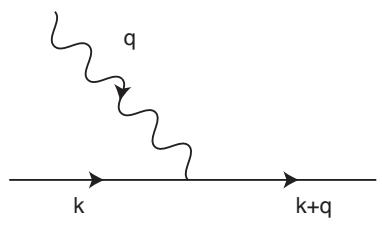
\includegraphics[width=0.48\textwidth]{figs/ch11/fig_11.1_a.jpg}\hfill
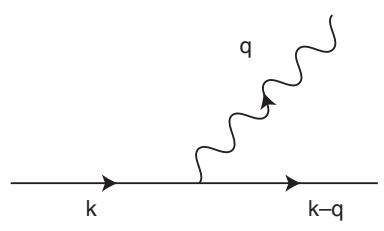
\includegraphics[width=0.48\textwidth]{figs/ch11/fig_11.1_b.jpg}\\[0.8em]
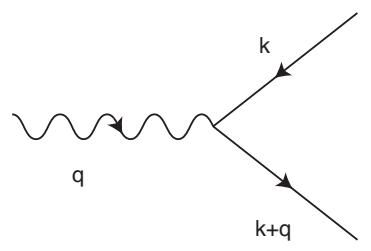
\includegraphics[width=0.48\textwidth]{figs/ch11/fig_11.1_c.jpg}\hfill
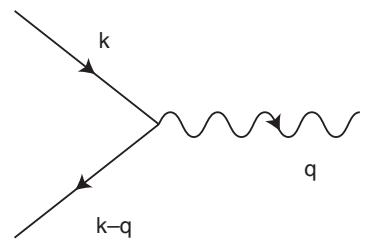
\includegraphics[width=0.48\textwidth]{figs/ch11/fig_11.1_d.jpg}
\caption*{图 11.1\quad 电子–声子散射。波浪线代表声子，入射与出射箭头分别代表电子与空穴。(a) 与 (c) 表示吸收，(b) 与 (d) 对应于发射一个声子。}\label{fig:auto:11.1}
\end{figure}

我们主要关心发射与吸收的振幅。发射时产生一个声子，因此只有 $b_{-\mathbf{q}}^{\dagger}$ 项有贡献；同样地，吸收时湮灭一个声子。对于发射过程，初态与末态必须具有形式
\begin{equation*}
|\mathrm{init}\rangle=|n_{\mathbf{k}+\mathbf{q}},n_{\mathbf{k}};N_{-\mathbf{q}},N_{\mathbf{q}}\rangle\tag{11.39}
\end{equation*}
与
\begin{equation*}
|\mathrm{efin}\rangle=|n_{\mathbf{k}+\mathbf{q}}+1,n_{\mathbf{k}}-1;N_{-\mathbf{q}}+1,N_{\mathbf{q}}\rangle.\tag{11.40}
\end{equation*}
发射振幅涉及矩阵元
\begin{equation*}
\langle\mathrm{efin}|H_{\text{e-ph}}|\mathrm{init}\rangle=M_{\mathbf{q}}\alpha_{\mathbf{k}+\mathbf{q},\mathbf{k}}\langle\mathrm{efin}|a_{\mathbf{q}+\mathbf{k}}^{\dagger}a_{\mathbf{k}}b_{-\mathbf{q}}^{\dagger}|\mathrm{init}\rangle.\tag{11.41}
\end{equation*}
因为 $n_{\mathbf{k}+\mathbf{q}}$ 与 $n_{\mathbf{k}}$ 被限制为 1 或 0，$a_{\mathbf{k}}|\mathrm{init}\rangle$ 仅当 $n_{\mathbf{k}}=1$ 时才非零。同样，$a_{\mathbf{q}+\mathbf{k}}^{\dagger}|\mathrm{init}\rangle$ 仅当 $1-n_{\mathbf{q}+\mathbf{k}}=1$ 时才给出非零结果。于是
\begin{equation*}
\langle\mathrm{efin}|H_{\text{e-ph}}|\mathrm{init}\rangle=M_{\mathbf{q}}\alpha_{\mathbf{k}+\mathbf{q},\mathbf{k}}\sqrt{(1-n_{\mathbf{q}+\mathbf{k}})n_{\mathbf{k}}(N_{-\mathbf{q}}+1)}.\tag{11.42}
\end{equation*}
当 $n_{\mathbf{k}}=1$ 且 $n_{\mathbf{q}+\mathbf{k}}=0$ 时，初态与末态的能量差为
\begin{equation*}
\Delta E_{\mathrm{emis}}=E_{\mathrm{fin}}-E_{\mathrm{init}}=E(\mathbf{q}+\mathbf{k})-E(\mathbf{k})+\hbar\omega_{\mathbf{q}},\tag{11.43}
\end{equation*}
其中 $E(\mathbf{k})$ 是动量为 $\mathbf{k}$ 的电子态的能量。

在吸收过程中，此时末态为
\begin{equation*}
|\mathrm{afin}\rangle=|n_{\mathbf{k}+\mathbf{q}}+1,n_{\mathbf{k}}-1;N_{-\mathbf{q}},N_{\mathbf{q}}-1\rangle.\tag{11.44}
\end{equation*}
于是
\begin{equation*}
\langle\mathrm{afin}|H_{\text{e-ph}}|\mathrm{init}\rangle=M_{\mathbf{q}}\alpha_{\mathbf{k}+\mathbf{q},\mathbf{k}}\sqrt{(1-n_{\mathbf{q}+\mathbf{k}})n_{\mathbf{k}}N_{\mathbf{q}}}.\tag{11.45}
\end{equation*}
此处能量差为
\begin{equation*}
\Delta E_{\mathrm{abs}}=E(\mathbf{k}+\mathbf{q})-E(\mathbf{k})-\hbar\omega_{\mathbf{q}}.\tag{11.46}
\end{equation*}
对发射与吸收振幅应用费米黄金定则（Fermi's golden rule），得到吸收与发射速率
\begin{equation*}
W^{\mathrm{abs}}_{\mathbf{k}\to\mathbf{k}+\mathbf{q}}=\frac{2\pi}{\hbar}|M_{\mathbf{q}}\alpha_{\mathbf{k}+\mathbf{q},\mathbf{k}}|^2 n_{\mathbf{k}}N_{\mathbf{q}}(1-n_{\mathbf{q}+\mathbf{k}})\delta(E(\mathbf{k}+\mathbf{q})-E(\mathbf{k})-\hbar\omega_{\mathbf{q}})\tag{11.47}
\end{equation*}
与
\begin{equation*}
W^{\mathrm{emis}}_{\mathbf{k}\to\mathbf{k}+\mathbf{q}}=\frac{2\pi}{\hbar}|M_{\mathbf{q}}\alpha_{\mathbf{k}+\mathbf{q},\mathbf{k}}|^2 n_{\mathbf{k}}(1-n_{\mathbf{q}+\mathbf{k}})(N_{-\mathbf{q}}+1)\delta(E(\mathbf{k}+\mathbf{q})-E(\mathbf{k})+\hbar\omega_{\mathbf{q}})\tag{11.48}
\end{equation*}
\footnote{译注：原书本句为“……for the emission and absorption rates, respectively”，其顺序与公式实际内容（式 (11.47) 为吸收、式 (11.48) 为发射）不符，已按公式本意译出。}。$\delta$ 函数保证能量守恒。为保持普遍性，我们显式写入了电子占据数，尽管实际上 $n_{\mathbf{k}}=1$、$n_{\mathbf{q}+\mathbf{k}}=0$。在计算的这一阶段，习惯上把电子与声子占据数换成平衡的费米–狄拉克与玻色形式。这一简化只有在电子–声子系统在跃迁发生前处于平衡时才有效。在处理超导电性时我们会发现这一简化很有用。

\section{超声衰减}

设想把一束声子射入金属。声子被吸收的总速率由直接被金属吸收与重新发射回束流两者共同决定。因此，束流单位时间损失 $N_{\mathbf{q},\lambda}$ 个声子的速率由一个动力学的增益–损耗方程给出：
\begin{equation*}
\frac{\mathrm{d}N_{\mathbf{q},\lambda}}{\mathrm{d}t}=-\sum_{\mathbf{p}}\bigl(W^{\mathrm{abs}}_{\mathbf{p}\to\mathbf{p}+\mathbf{q}}-W^{\mathrm{emis}}_{\mathbf{p}\to\mathbf{p}-\mathbf{q}}\bigr).\tag{11.49}
\end{equation*}
第一项代表从束流中吸收声子，第二项代表声子再发射回束流。要正确描述物理，把再发射项包括进来是必不可少的。

回忆自由电子的结构函数为
\begin{equation*}
n_{\mathrm{e}}S_0(\mathbf{p},\omega)=\frac{2}{V}\sum_{\mathbf{p}'}f_{\mathbf{p}'}(1-f_{\mathbf{p}+\mathbf{p}'})2\pi\hbar\delta(\hbar\omega-\epsilon_{\mathbf{p}+\mathbf{p}'}+\epsilon_{\mathbf{p}'}).\tag{11.50}
\end{equation*}
据此可简化上述动力学方程。物理上，$S_0(\mathbf{p},\omega)$ 是能量间隔为 $\hbar\omega$ 的电子–空穴激发的密度。查看声子吸收与发射速率的表达式可以发现，它们正比于结构函数方程的右端。我们假设电子态是具有自由粒子能量 $\epsilon_{\mathbf{p}}=\mathbf{p}^2/2m$ 的完美平面波。于是，式 (11.37) 中的矩阵元等于 1：$\alpha_{\mathbf{k}+\mathbf{q},\mathbf{q}}=1$。据此，我们把净吸收与发射速率改写为
\begin{equation*}
\sum_{\mathbf{p}}W^{\mathrm{abs}}_{\mathbf{p}\to\mathbf{p}+\mathbf{q}}=\frac{n_{\mathrm{e}}V}{2\hbar^2}|M_{\mathbf{q}}|^2 N_{\mathbf{q},\lambda}S_0(\mathbf{q},\hbar\omega_{\mathbf{q}})\tag{11.51}
\end{equation*}
与
\begin{equation*}
\sum_{\mathbf{p}}W^{\mathrm{emis}}_{\mathbf{p}\to\mathbf{p}-\mathbf{q}}=\frac{n_{\mathrm{e}}V}{2\hbar^2}|M_{\mathbf{q}}|^2(N_{\mathbf{q},\lambda}+1)S_0(-\mathbf{q},-\hbar\omega_{\mathbf{q}}).\tag{11.52}
\end{equation*}
在涨落–耗散定理的语境中，我们曾证明
\begin{equation*}
S_0(\mathbf{p},\hbar\omega)=\mathrm{e}^{\beta\hbar\omega}S_0(-\mathbf{p},-\hbar\omega).\tag{11.53}
\end{equation*}
将此结果代入 $N_{\mathbf{q},\lambda}(t)$ 的运动方程，得到
\begin{equation*}
\dot{N}_{\mathbf{q},\lambda}=-\frac{n_{\mathrm{e}}V}{2\hbar^2}|M_{\mathbf{q}}|^2 S_0(\mathbf{q},\omega_{\mathbf{q}}\hbar)\bigl[N_{\mathbf{q},\lambda}-\mathrm{e}^{-\beta\hbar\omega_{\mathbf{q}}}(N_{\mathbf{q},\lambda}+1)\bigr].\tag{11.54}
\end{equation*}
我们定义声子的净吸收速率为
\begin{equation*}
\frac{1}{\tau_{\mathrm{ph}}}=\frac{n_{\mathrm{e}}V}{2\hbar^2}|M_{\mathbf{q}}|^2(1-\mathrm{e}^{-\beta\hbar\omega_{\mathbf{q}}})S_0(\mathbf{q},\hbar\omega_{\mathbf{q}})\tag{11.55}
\end{equation*}
并把平衡声子分布 $N^{\mathrm{eq}}_{\mathbf{q},\lambda}$ 取为标准的玻色–爱因斯坦分布函数
\begin{equation*}
N^{\mathrm{eq}}_{\mathbf{q},\lambda}=\frac{1}{\mathrm{e}^{\beta\hbar\omega_{\mathbf{q}}}-1}.\tag{11.56}
\end{equation*}
于是，我们的运动方程化为
\begin{equation*}
\dot{N}_{\mathbf{q},\lambda}=\frac{-1}{\tau_{\mathrm{ph}}}\bigl[N_{\mathbf{q},\lambda}-N^{\mathrm{eq}}_{\mathbf{q},\lambda}\bigr],\tag{11.57}
\end{equation*}
而这个线性微分方程的解具有
\begin{equation*}
N_{\mathbf{q},\lambda}(t)=N^{\mathrm{eq}}_{\mathbf{q},\lambda}+\mathrm{e}^{-t/\tau_{\mathrm{ph}}}\bigl(N_{\mathbf{q},\lambda}(t=0)-N^{\mathrm{eq}}_{\mathbf{q},\lambda}\bigr)\tag{11.58}
\end{equation*}
的特征指数形式。于是我们发现，被吸收声子数在长时间后以 $1/\tau_{\mathrm{ph}}$ 的速率弛豫到平衡值。这一效应称为超声衰减（ultrasonic attenuation），即声子因与电子相互作用而被介质损耗。超导体中的电子成对地束缚在一起，结合能正比于能隙，因此只有当声子频率超过某个临界值时它们才能吸收声子。因而超声衰减被用作测量超导体能隙的工具。我们将在下一章进一步讨论这一点。

最后指出一点：我们在这里进行的计算仅在电子相互作用可以忽略时才有效。也就是说，若 $\tau_{\mathrm{ee}}$ 是电子散射的有效时标，则当 $\omega_{\mathbf{q}}\tau_{\mathrm{ee}}\gg 1$ 时我们的计算有效。若该条件不成立，即 $\tau_{\mathrm{ee}}\omega_{\mathbf{q}}<1$，则声波经由电子散射而非声子诱导的电子–空穴对而衰减。为完整起见，现在来计算 $\tau_{\mathrm{ph}}$。在 $T=0$ 处我们曾证明，在中间频段 $n_{\mathrm{e}}S_0(\mathbf{k},\omega)=m^2\omega/\pi k\hbar^2$。由于 $|M_{\mathbf{q}}|^2\sim q^2|V_{\mathrm{ei}}(\mathbf{q})|^2/\omega_{\mathbf{q}}$，故 $1/\tau_{\mathrm{ph}}\sim q|V_{\mathrm{ei}}(\mathbf{q})|^2$。只关注结构函数的零频部分，我们发现 $\epsilon_{\mathbf{p}}=\epsilon_{\mathbf{p}+\mathbf{k}}$。对 $p=p_{\mathrm{F}}$，转移的动量为 $k=2p_{\mathrm{F}}$。因此，在低频下，$\tau_{\mathrm{ph}}$ 由横跨费米面的粒子散射决定。

\section{电传导}

金属的电导率通过在材料上施加电压或电场来测量。由此产生的电流密度
\begin{equation*}
\mathbf{j}=\sigma\mathbf{E}\tag{11.59}
\end{equation*}
通过电导率 $\sigma$ 与电场直接成正比。电流密度沿载流子速度 $\mathbf{v}$ 的方向，比例常数是净电荷密度 $-en_{\mathrm{e}}$。因此
\begin{equation*}
\mathbf{j}=-n_{\mathrm{e}}e\mathbf{v}.\tag{11.60}
\end{equation*}
现在把 $\mathbf{v}$ 用 $\mathbf{E}$ 表达。没有电场时，$\langle\mathbf{v}\rangle=0$，因为 $\mathbf{v}$ 是无规的。令 $\tau$ 为电子的碰撞时间。也就是说，在一段时长 $\tau$ 内，电子以恒定速度运动，我们估计如下。电场施加在电子上的力就是 $-e\mathbf{E}$，于是电子的加速度为 $-e\mathbf{E}/m$。若加速度在时间 $\tau$ 内恒定，则平均速度为 $\mathbf{v}_{\mathrm{avg}}=-e\mathbf{E}\tau/m$，电流密度为
\begin{equation*}
\mathbf{j}=\frac{e^2n_{\mathrm{e}}}{m}\mathbf{E}\tau=\sigma\mathbf{E}\tag{11.61}
\end{equation*}
或者等价地
\begin{equation*}
\sigma=\frac{n_{\mathrm{e}}e^2\tau}{m}.\tag{11.62}
\end{equation*}
这就是电导率的德鲁德（Drude）公式。

于是我们把电导率用单一的未知量 $\tau$——弛豫时间或碰撞时间——表达了出来。实验上，一旦测得电导率，便可提取 $\tau$。表11.1列出了碱金属的几个弛豫时间（文献 [AM1976]）\footnote{译注：原文为“alkali earth metals”（碱土金属），但表中所列的 Li、Na、K、Rb、Cs 均为碱金属，现按表的内容译出。}。现在我们想发展一个能够解释弛豫时间进而解释电导率的普遍理论。在纯金属中，电阻的主要来源是与晶格声子的相互作用。任何关于金属中 $\sigma$ 的成功解释都必须说明以下几点：(1) 在 $\mathbf{E}$ 取中等数值时 $\sigma$ 与 $\mathbf{E}$ 无关；(2) $\sigma$ 在不同金属之间变化巨大；(3) 维德曼–弗兰兹定律（Wiedemann--Franz law），即比值 $\kappa/\sigma=T$，其中 $\kappa$ 是热导率；(4) 大多数金属中 $\sigma\sim 1/T$，且在 $T\to 0$ 时过渡到 $\sigma\sim T^{-5}$。本章完全关注低温下从 $1/T$ 到 $T^{-5}$ 行为的交叉过渡。

\begin{center}
表 11.1

\begin{tabular}{lcc}
\toprule
元素 & 77 K & 273 K\\
\midrule
Li & $7.3\times 10^{-14}\,\mathrm{s}$ & $8.8\times 10^{-15}\,\mathrm{s}$\\
Na & $1.7\times 10^{-13}\,\mathrm{s}$ & $3.2\times 10^{-14}\,\mathrm{s}$\\
K & $1.8\times 10^{-13}\,\mathrm{s}$ & $4.1\times 10^{-14}\,\mathrm{s}$\\
Rb & $1.4\times 10^{-13}\,\mathrm{s}$ & $2.8\times 10^{-14}\,\mathrm{s}$\\
Cs & $8.6\times 10^{-14}\,\mathrm{s}$ & $2.1\times 10^{-14}\,\mathrm{s}$\\
\bottomrule
\end{tabular}
\end{center}

\subsection{玻尔兹曼方程}

为此我们发展玻尔兹曼输运理论。引入分布函数 $f(\mathbf{r},\mathbf{k},t)$，它定义为时刻 $t$ 动量为 $\mathbf{k}$、位置为 $\mathbf{r}$ 的一个量子“态”被占据的概率。虽然我们只关心一个能带，$f$ 可以推广到包括固体中的所有能带。分布函数 $f$ 同时给定量子态中电子的位置和动量。严格说来，采用这样的分布函数只在长波长下有效，即 $\lambda\gg\hbar v_{\mathrm{F}}/\kappa_{\mathrm{B}}T$。否则将违反不确定性原理。

考虑体积元 $\mathrm{d}\mathbf{k}\,\mathrm{d}\mathbf{r}/(2\pi\hbar)^3=\mathrm{d}\Omega$。该微分体积元与 $f$ 的乘积 $f\,\mathrm{d}\Omega$ 定义了 $\mathrm{d}\Omega$ 中的电子数。在眼前的问题中，与声子的相互作用改变相空间中的占据。我们把这类过程称为晶格碰撞。显然，若无此类碰撞，$\mathrm{d}f/\mathrm{d}t$ 将为零。事实上，对处于平衡的固体，$f$ 就是费米–狄拉克分布。对非平衡情形，$f$ 必须由普遍的运动方程确定。$f$ 的全时间导数
\begin{equation*}
\frac{\mathrm{d}f}{\mathrm{d}t}=\frac{\partial f}{\partial t}+\dot{\mathbf{k}}\cdot\nabla_{\mathbf{k}}f+\dot{\mathbf{r}}\cdot\nabla_{\mathbf{r}}f=\left.\frac{\partial f}{\partial t}\right|_{\mathrm{coll}},\tag{11.63}
\end{equation*}
由所有隐式或显式依赖时间的项决定。这就是玻尔兹曼方程（Boltzmann equation）。因为每个体积元应当等价，进入与离开某个体积元的电子平均数应为常数。于是 $\partial f/\partial t=0$。此外，即使存在电场，我们的系统仍是均匀的。因此，$f$ 的空间导数为零，得到
\begin{equation*}
\left.\frac{\partial\mathbf{k}}{\partial t}\cdot\nabla_{\mathbf{k}}f=\frac{\partial f}{\partial t}\right|_{\mathrm{coll}},\tag{11.64}
\end{equation*}
即稳态玻尔兹曼方程。物理上，$\partial\mathbf{k}/\partial t$ 是作用于费米海中电子的力。存在电场时，
\begin{equation*}
\frac{\partial\mathbf{k}}{\partial t}=-e\mathbf{E},\tag{11.65}
\end{equation*}
因而所有电子被电场同等地加速。

\begin{figure}[H]\centering
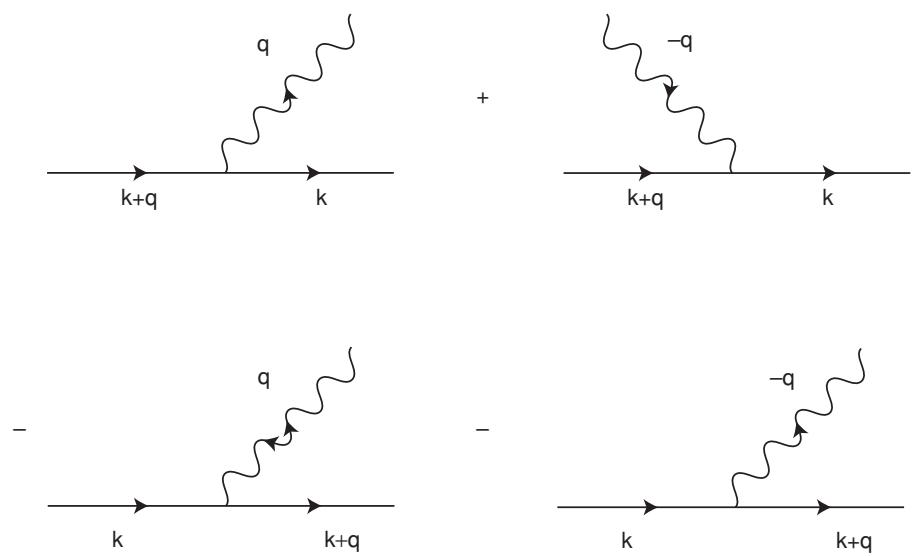
\includegraphics[width=0.8\textwidth]{figs/ch11/fig_11.2.jpg}
\caption*{图 11.2\quad 进入玻尔兹曼方程的电子–声子碰撞项。}\label{fig:auto:11.2}
\end{figure}

要把这个方程应用于电子–晶格问题，必须为声子引入一个类似的玻尔兹曼方程。合适的玻尔兹曼方程不含动量项，因为在无应变的晶体中声子不受力。令 $g$ 为声子分布函数，则有
\begin{equation*}
\left.\frac{\partial g}{\partial t}\right|_{\mathrm{coll}}=\dot{\mathbf{r}}\cdot\nabla_{\mathbf{r}}g.\tag{11.66}
\end{equation*}
在接下来的所有计算中，我们都将用 $g$ 的平衡值代替它，因此不必多费笔墨讨论 $g$，尽管对 $f$ 的处理可以平行地用来求解 $g$。因为 $f$ 由电子–声子交换决定，我们能写出的最普遍的碰撞表达式是对所有可能的电子–声子过程求和。令 $W^{e\mathbf{q}}$ 表示发射项，$W^{a\mathbf{q}}$ 表示波矢为 $\mathbf{q}$ 的声子吸收过程。进入玻尔兹曼方程的一般碰撞项如图11.2所示，可以写成增益–损耗主方程
\begin{align*}
\left.\frac{\partial f}{\partial t}\right|_{\mathrm{coll}}&=\sum_{\mathbf{q}}\bigl(W^{e\mathbf{q}}_{\mathbf{k}+\mathbf{q}\to\mathbf{k}}+W^{a\mathbf{-q}}_{\mathbf{k}+\mathbf{q}\to\mathbf{k}}-W^{a\mathbf{q}}_{\mathbf{k}\to\mathbf{k}+\mathbf{q}}-W^{e\mathbf{-q}}_{\mathbf{k}\to\mathbf{k}+\mathbf{q}}\bigr)\\
&=\sum_{\mathbf{q}}[\mathrm{gain}(\mathbf{k})-\mathrm{loss}(\mathbf{k})],\tag{11.67}
\end{align*}
其中电子态的动量为 $\mathbf{k}$ 与 $\mathbf{k}+\mathbf{q}$。利用式 (11.47) 与式 (11.48) 中 $W$ 的精确表达式，方便的做法是定义
\begin{equation*}
W^0_{\mathbf{q}}=\frac{2\pi}{\hbar}|M_{\mathbf{q}}|^2.\tag{11.68}
\end{equation*}
我们已经假定电子态是平面波，因此 $\alpha_{\mathbf{k},\mathbf{q}}=1$。若把式 (11.68) 中的碰撞项按发射–吸收对分组，则容易计算：
\begin{align*}
\left.\frac{\partial f}{\partial t}\right|_{\mathrm{coll}}&=\sum_{\mathbf{q}}\bigl(W^{e\mathbf{q}}_{\mathbf{k}+\mathbf{q}\to\mathbf{k}}-W^{a\mathbf{q}}_{\mathbf{k}\to\mathbf{k}+\mathbf{q}}\bigr)-\bigl(W^{e\mathbf{-q}}_{\mathbf{k}\to\mathbf{k}+\mathbf{q}}-W^{a\mathbf{-q}}_{\mathbf{k}+\mathbf{q}\to\mathbf{k}}\bigr)\\
&=\sum_{\mathbf{q}}W^0_{\mathbf{q}}\bigl[(1-f(\mathbf{k}))f(\mathbf{k}+\mathbf{q})(g(\mathbf{q})+1)\delta(\epsilon_{\mathbf{k}}-\epsilon_{\mathbf{k}+\mathbf{q}}+\hbar\omega_{\mathbf{q}})\\
&\quad -(1-f(\mathbf{k}+\mathbf{q}))f(\mathbf{k})g(\mathbf{q})\delta(\epsilon_{\mathbf{k}+\mathbf{q}}-\epsilon_{\mathbf{k}}-\hbar\omega_{\mathbf{q}})\bigr]\\
&\quad +W^0_{\mathbf{q}}\bigl[(1-f(\mathbf{k}))f(\mathbf{k}+\mathbf{q})g(-\mathbf{q})\delta(\epsilon_{\mathbf{k}}-\epsilon_{\mathbf{k}+\mathbf{q}}-\hbar\omega_{\mathbf{q}})\\
&\quad -(1-f(\mathbf{k}+\mathbf{q}))f(\mathbf{k})(g(-\mathbf{q})+1)\delta(\epsilon_{\mathbf{k}+\mathbf{q}}-\epsilon_{\mathbf{k}}+\hbar\omega_{\mathbf{q}})\bigr].\tag{11.69}
\end{align*}

求解 $f(\mathbf{k})$ 的玻尔兹曼方程常用三种简化。第一种是假定 $g(\mathbf{q})=g_{\mathrm{equil}}$，这称为布洛赫假定（Bloch assumption）。玻色–爱因斯坦分布正是 $g_{\mathrm{equil}}$。令 $N_{\mathbf{q}}=g_{\mathrm{equil}}=N_{-\mathbf{q}}$。我们还定义
\begin{equation*}
W_{\mathbf{q}}(\mathbf{k},\mathbf{k}')=W^0_{\mathbf{q}}\bigl[\delta(\epsilon_{\mathbf{k}'}-\epsilon_{\mathbf{k}}+\hbar\omega_{\mathbf{q}})(N_{\mathbf{q}}+1)+N_{\mathbf{q}}\delta(\epsilon_{\mathbf{k}'}-\epsilon_{\mathbf{k}}-\hbar\omega_{\mathbf{q}})\bigr].
\end{equation*}
玻尔兹曼方程的右端于是简化为
\begin{equation*}
\left.\frac{\partial f}{\partial t}\right|_{\mathrm{coll}}=\sum_{\mathbf{q}}\bigl[W_{\mathbf{q}}(\mathbf{k}+\mathbf{q},\mathbf{k})f(\mathbf{k}+\mathbf{q})(1-f(\mathbf{k}))-W_{\mathbf{q}}(\mathbf{k},\mathbf{k}+\mathbf{q})f(\mathbf{k})(1-f(\mathbf{k}+\mathbf{q}))\bigr].\tag{11.70}
\end{equation*}

\subsection{弛豫时间近似}

下一步，我们假设施加电场后 $f(\mathbf{k})$ 平均而言缓变。与声子的碰撞使系统回到平衡的费米–狄拉克分布函数 $f_0=n_{\mathbf{k}}$。我们把 $f(\mathbf{k})$ 写成
\begin{equation*}
f(\mathbf{k})\simeq n_{\mathbf{k}}+\delta f_{\mathbf{k}},\tag{11.71}
\end{equation*}
其中 $\delta f_{\mathbf{k}}$ 是电场引起的 $f(\mathbf{k})$ 的变化。我们猜测 $\delta f_{\mathbf{k}}$ 正比于加速度 $\partial\mathbf{k}/\partial t$。为看清个中缘由，我们作如下拟设：碰撞引起的 $f(\mathbf{k})$ 的变化以平均弛豫时间 $\tau(\mathbf{k})$ 把系统弛豫回 $n_{\mathbf{k}}$，使得
\begin{equation*}
\left.\frac{\partial f}{\partial t}\right|_{\mathrm{coll}}=-\frac{\delta f_{\mathbf{k}}}{\tau(\mathbf{k})}.\tag{11.72}
\end{equation*}
注意，在此阶段引入弛豫时间的代价是 $\tau$ 必须依赖 $\mathbf{k}$。利用式 (11.64) 与式 (11.65)，并对涨落 $\delta f_{\mathbf{k}}$ 线性化，我们得到
\begin{align*}
\left.\frac{\partial f}{\partial t}\right|_{\mathrm{coll}}&=-\frac{\delta f_{\mathbf{k}}}{\tau}=-e\mathbf{E}\cdot\nabla_{\mathbf{k}}f(\mathbf{k})\\
&=-e\mathbf{E}\cdot\nabla_{k}\epsilon_{\mathbf{k}}\frac{\partial n_{\mathbf{k}}}{\partial\epsilon_{\mathbf{k}}}\\
&=e\,\frac{\mathbf{E}\cdot\mathbf{k}}{m}\,n_{\mathbf{k}}(1-n_{\mathbf{k}})\beta,\tag{11.73}
\end{align*}
其中我们用了自由粒子色散关系 $\epsilon_{\mathbf{k}}=\mathbf{k}^2/2m$。由于 $\delta f_{\mathbf{k}}=f(\mathbf{k})-n_{\mathbf{k}}$，我们得到
\begin{equation*}
f(\mathbf{k})=n_{\mathbf{k}}+\beta\delta\Phi_{\mathbf{k}}n_{\mathbf{k}}(1-n_{\mathbf{k}}),\tag{11.74}
\end{equation*}
其中
\begin{equation*}
\delta\Phi_{\mathbf{k}}=-e\,\frac{\mathbf{E}\cdot\mathbf{k}}{m}\,\tau(\mathbf{k}).\tag{11.75}
\end{equation*}
我们看到，一旦确定了 $\tau(\mathbf{k})$，便可立即得到分布函数 $f(\mathbf{k})$，并经由德鲁德公式求出电导率。

\subsection{低温电阻率}

为简化玻尔兹曼方程，我们注意到 $W_{\mathbf{q}}(\mathbf{k},\mathbf{k}')$ 满足对称关系
\begin{equation*}
W_{\mathbf{q}}(\mathbf{k},\mathbf{k}')\mathrm{e}^{\beta\epsilon_{\mathbf{k}'}}=W_{\mathbf{q}}(\mathbf{k}',\mathbf{k})\mathrm{e}^{\beta\epsilon_{\mathbf{k}}}.\tag{11.76}
\end{equation*}
这个表述其实就是细致平衡（detailed balance）。式 (11.76) 的一个等价且更有用的写法是
\begin{align*}
W_{\mathbf{q}}(\mathbf{k},\mathbf{k}')&=\mathrm{e}^{\beta(\epsilon_{\mathbf{k}}-\epsilon_{\mathbf{k}'})}W_{\mathbf{q}}(\mathbf{k}',\mathbf{k})\tag{11.77}\\
&=\frac{n_{\mathbf{k}'}(1-n_{\mathbf{k}})}{n_{\mathbf{k}}(1-n_{\mathbf{k}'})}W_{\mathbf{q}}(\mathbf{k}',\mathbf{k}).\tag{11.78}
\end{align*}
这个恒等式意味着，量
\begin{equation*}
Z_{\mathbf{q}}(\mathbf{k},\mathbf{k}')=W_{\mathbf{q}}(\mathbf{k},\mathbf{k}')n_{\mathbf{k}}(1-n_{\mathbf{k}'})\tag{11.79}
\end{equation*}
对其宗量的互换是对称的。该恒等式的一个直接推论是：当 $f(\mathbf{k})=n_{\mathbf{k}}$ 时，玻尔兹曼方程中的碰撞项恒等地变为零：

\begin{figure}[H]\centering
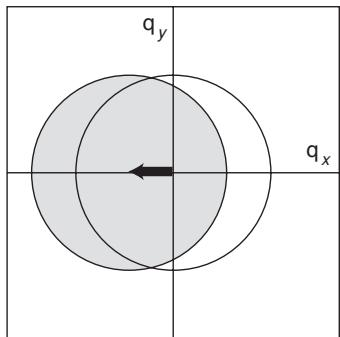
\includegraphics[width=0.42\textwidth]{figs/ch11/fig_11.3.jpg}
\caption*{图 11.3\quad 平衡费米面与存在均匀电场时的费米面。漂移速度拟设断言：一旦加上电场，新的费米–狄拉克分布函数等价于把原来的分布作平移 $\mathbf{q}\to\mathbf{q}-m\mathbf{v}_{\mathrm{d}}$。}\label{fig:auto:11.3}
\end{figure}

\begin{align*}
&W_{\mathbf{q}}(\mathbf{k}',\mathbf{k})(1-n_{\mathbf{k}})n_{\mathbf{k}'}-W_{\mathbf{q}}(\mathbf{k},\mathbf{k}')(1-n_{\mathbf{k}'})n_{\mathbf{k}}=Z_{\mathbf{q}}(\mathbf{k}',\mathbf{k})-Z_{\mathbf{q}}(\mathbf{k},\mathbf{k}')\\
&=0.\tag{11.80}
\end{align*}
这一恒等式的后果立竿见影。回忆我们把 $f(\mathbf{k})$ 近似为 $f(\mathbf{k})\simeq n_{\mathbf{k}}+\beta n_{\mathbf{k}}(1-n_{\mathbf{k}})\delta\Phi_{\mathbf{k}}$。因此，玻尔兹曼方程中只有至少含 $\delta f$ 一次变分的项存活下来：
\begin{align*}
\left.\frac{\partial f}{\partial t}\right|_{\mathrm{coll}}&=\sum_{\mathbf{q}}W_{\mathbf{q}}(\mathbf{k}',\mathbf{k})\bigl(\delta f_{\mathbf{k}'}(1-n_{\mathbf{k}})-n_{\mathbf{k}'}\delta f_{\mathbf{k}}\bigr)-(\mathbf{k}\Leftrightarrow\mathbf{k}')\\
&=\beta\sum_{\mathbf{q}}Z_{\mathbf{q}}(\mathbf{k}',\mathbf{k})\bigl[\delta\Phi_{\mathbf{k}'}(1-n_{\mathbf{k}'})-\delta\Phi_{\mathbf{k}}n_{\mathbf{k}}-(\mathbf{k}\Leftrightarrow\mathbf{k}')\bigr]\\
&=\beta\sum_{\mathbf{q}}Z_{\mathbf{q}}(\mathbf{k}',\mathbf{k})\bigl[\delta\Phi_{\mathbf{k}'}-\delta\Phi_{\mathbf{k}}\bigr].\tag{11.81}
\end{align*}
在推导式 (11.81) 时，我们略去了 $O(\delta\Phi^2)$ 项，从而得到线性化的玻尔兹曼方程。

由于变分 $\delta\Phi_{\mathbf{k}}\sim\tau(\mathbf{k})$，玻尔兹曼方程一般是一个积分方程，必须通过某个拟设自洽地求解。与所有积分方程一样，这里适用一个变分原理：可以保证，$\delta\Phi$ 的试探解所给出的分布函数 $f$ 的能量高于真实基态能量。在弛豫时间近似中，$\delta\Phi_{\mathbf{k}}=-e\mathbf{E}\cdot\mathbf{k}\tau(\mathbf{k})/m$。电场中的漂移速度为 $\mathbf{v}_{\mathrm{d}}=-e\mathbf{E}\tau/m$。因此，$\delta\Phi_{\mathbf{k}}\equiv\mathbf{v}_{\mathrm{d}}\cdot\mathbf{k}$ 称为漂移速度拟设（drift velocity ansatz）。物理上，该拟设表示电子与一个漂移的分布处于平衡。这个漂移分布等价于对平衡费米–狄拉克分布作替换 $\mathbf{q}\to\mathbf{q}-m\mathbf{v}_{\mathrm{d}}$。如图11.3所示，漂移速度拟设相当于把费米面整体平移一个（线性阶）正比于 $m\mathbf{v}_{\mathrm{d}}$ 的量。我们对碰撞项作电子动量平均，从而封闭玻尔兹曼方程：
\begin{align*}
\left.\frac{\partial}{\partial t}\langle\mathbf{k}\rangle\right|_{\mathrm{coll}}&=2\int\mathbf{k}\left.\frac{\partial f}{\partial t}\right|_{\mathrm{coll}}\frac{\mathrm{d}\mathbf{k}}{(2\pi\hbar)^3}\\
&=-2\int\mathbf{k}\,\frac{\mathrm{d}\mathbf{k}}{(2\pi\hbar)^3}\,\frac{f-f_0}{\tau}\\
&=-2\int\mathbf{k}\,\frac{\mathrm{d}\mathbf{k}}{(2\pi\hbar)^3}\,\frac{f_0(\mathbf{k}-m\mathbf{v}_{\mathrm{d}})}{\tau}\\
&=-\frac{m\mathbf{v}_{\mathrm{d}}n_{\mathrm{e}}}{\tau}.\tag{11.82}
\end{align*}
在推导式 (11.82) 时，我们用了 $\langle\mathbf{k}\rangle$ 在平衡时为零这一事实。

注意到碰撞项在 $\mathbf{k}$ 与 $\mathbf{k}'$ 互换下是反对称的，把式 (11.82) 代入玻尔兹曼方程，我们得到
\begin{align*}
\frac{-m\mathbf{v}_{\mathrm{d}}n_{\mathrm{e}}}{\tau}&=\frac{\beta}{V}\sum_{\mathbf{k}}\mathbf{k}\sum_{\mathbf{k}'}W_{\mathbf{q}}(\mathbf{k},\mathbf{k}')n_{\mathbf{k}}(1-n_{\mathbf{k}'})[\mathbf{v}_{\mathrm{d}}\cdot\mathbf{k}'-\mathbf{v}_{\mathrm{d}}\cdot\mathbf{k}]\\
&=\frac{\beta}{2V}\sum_{\mathbf{k}}\sum_{\mathbf{k}'}(\mathbf{k}-\mathbf{k}')W_{\mathbf{q}}(\mathbf{k},\mathbf{k}')n_{\mathbf{k}}(1-n_{\mathbf{k}'})[\mathbf{v}_{\mathrm{d}}\cdot\mathbf{k}'-\mathbf{v}_{\mathrm{d}}\cdot\mathbf{k}]\\
&=-\frac{\beta}{2V}\sum_{\mathbf{k}}\sum_{\mathbf{q}}\mathbf{q}(\mathbf{v}_{\mathrm{d}}\cdot\mathbf{q})W^0_{\mathbf{q}}n_{\mathbf{k}}(1-n_{\mathbf{k}+\mathbf{q}})[\delta(\epsilon_{\mathbf{k}+\mathbf{q}}-\epsilon_{\mathbf{k}}+\hbar\omega_{\mathbf{q}})\\
&\quad\times(N_{\mathbf{q}}+1)+N_{\mathbf{q}}\delta(\epsilon_{\mathbf{k}+\mathbf{q}}-\epsilon_{\mathbf{k}}-\hbar\omega_{\mathbf{q}})],\tag{11.83}
\end{align*}
其中 $\mathbf{k}'=\mathbf{k}+\mathbf{q}$。回忆自由粒子结构函数的定义（见式 (11.50)），我们把线性化的玻尔兹曼方程约化为
\begin{align*}
\frac{m\mathbf{v}_{\mathrm{d}}n_{\mathrm{e}}}{\tau}&=\frac{n_{\mathrm{e}}\beta}{8\pi\hbar}\sum_q\mathbf{q}(\mathbf{v}_{\mathrm{d}}\cdot\mathbf{q})W^0_{\mathbf{q}}[S_0(\mathbf{q},\hbar\omega_{\mathbf{q}})N_{\mathbf{q}}+(N_{\mathbf{q}}+1)S_0(\mathbf{q},-\hbar\omega_{\mathbf{q}})]\\
&=\frac{n_{\mathrm{e}}\beta}{4\pi\hbar}\sum_q\mathbf{q}(\mathbf{v}_{\mathrm{d}}\cdot\mathbf{q})W^0_{\mathbf{q}}N_{\mathbf{q}}S_0(\mathbf{q},\hbar\omega_{\mathbf{q}}).\tag{11.84}
\end{align*}
为进一步简化式 (11.84)，我们把 $\mathbf{q}(\mathbf{v}_{\mathrm{d}}\cdot\mathbf{q})$ 换成它的角平均
\begin{equation*}
\langle\mathbf{q}(\mathbf{q}\cdot\mathbf{v}_{\mathrm{d}})\rangle=\frac{1}{3}q^2\mathbf{v}_{\mathrm{d}}.\tag{11.85}
\end{equation*}
将式 (11.85) 代入式 (11.84)，得到弛豫时间的一般表达式
\begin{equation*}
\frac{1}{\tau}=\frac{\beta}{24\pi^2M\hbar^3mn_{\mathrm{ion}}}\int_0^{q_{\mathrm{D}}}\frac{q^6\,\mathrm{d}q}{\hbar\omega_{\mathbf{q}}}\,|V_{\mathrm{ei}}(q)|^2\,\frac{S_0(q,\hbar\omega_{\mathbf{q}})}{\mathrm{e}^{\beta\hbar\omega_{\mathbf{q}}}-1}\tag{11.86}
\end{equation*}
式 (11.86) 中，$q_{\mathrm{D}}$ 是声子谱的动量截断。

我们需要一个能在低温下抓住本质物理的 $S_0$ 表达式。我们在上一章证明过，$T=0$ 时 $S_0\propto 1/q$。渐近地，该表达式在 $q\to\infty$ 时趋于零，因此只要声子动量被截断，它就预期有效。弛豫时间中的德拜截断为我们使用 $T=0$ 极限提供了正当性。偏离 $T=0$ 时，可以通过纳入因子 $(1-\exp(-\beta\hbar\omega_{\mathbf{q}}))$——它出现在 $S_0(k,\omega)$ 的原始定义中——引入显式的温度依赖。于是我们写出
\begin{equation*}
S_0(q,\hbar\omega_{\mathbf{q}})=\frac{m^2\hbar\omega_{\mathbf{q}}}{\pi n_{\mathrm{e}}q\hbar^2(1-\mathrm{e}^{-\beta\hbar\omega_{\mathbf{q}}})}.\tag{11.87}
\end{equation*}
我们还需要 $V_{\mathrm{ei}}(q)$ 的表达式。在屏蔽的托马斯–费米（Thomas--Fermi）处理中，我们证明过
\begin{equation*}
V_{\mathrm{ei}}(q)=-\frac{4\pi Ze^2}{V(q^2+\kappa_{\mathrm{TF}}^2)}.\tag{11.88}
\end{equation*}
低温下，我们关注 $V_{\mathrm{ei}}$ 的 $(q\to 0)$ 极限。因此，我们用
\begin{equation*}
\begin{aligned}
V_{\mathrm{ei}}(q)&=-\frac{4\pi Ze^2}{V\kappa_{\mathrm{TF}}^2}\\
&=-\frac{\pi^2Z\hbar^3}{Vmp_{\mathrm{F}}}=-\frac{Z}{N(\epsilon_{\mathrm{F}})}.
\end{aligned}\tag{11.89}
\end{equation*}
来近似 $V_{\mathrm{ei}}(q)$。弛豫时间可以写成
\begin{equation*}
\frac{1}{\tau}=\frac{Z^2\beta m}{24\pi^3 n_{\mathrm{e}}\hbar^3N^2(\epsilon_{\mathrm{F}})Mn_{\mathrm{ion}}}\int_0^{q_{\mathrm{D}}}\frac{q^5\,\mathrm{d}q}{(1-\mathrm{e}^{-\beta\hbar\omega_{\mathbf{q}}})(\mathrm{e}^{\beta\hbar\omega_{\mathbf{q}}}-1)}.\tag{11.90}
\end{equation*}
对声子谱，我们使用线性色散关系 $w_q=sq/\hbar$，其中 $s$ 是常数。令 $x=\beta\omega_q$。\footnote{译注：原书此处印作 $w_q=sq/\hbar$ 与 $x=\beta\omega_q$；按上下文（式 (11.92) 的积分上限与指数），二者应分别为 $\omega_q=sq/\hbar$ 与 $x=\beta\hbar\omega_q$，正文照录原书。}利用观察
\begin{equation*}
\frac{1}{(\mathrm{e}^x-1)(1-\mathrm{e}^{-x})}=-\frac{\partial}{\partial x}\frac{1}{\mathrm{e}^x-1},\tag{11.91}
\end{equation*}
我们把弛豫时间改写为
\begin{align*}
\frac{1}{\tau}&=-\frac{Z^2\beta m}{24\pi^3\hbar^7 n_{\mathrm{e}}MN^2(\epsilon_{\mathrm{F}})(\beta s)^6}\int_0^{q_{\mathrm{D}}s\hbar/k_{\mathrm{B}}T}x^5\frac{\partial}{\partial x}\frac{\mathrm{d}x}{(\mathrm{e}^x-1)}\\
&=\alpha_0T^5J_5(T_{\mathrm{D}}/T),\tag{11.92}
\end{align*}
其中
\begin{equation*}
J_5(y)=-\int_0^y x^5\,\mathrm{d}x\,\frac{\partial}{\partial x}\frac{1}{\mathrm{e}^x-1},\tag{11.93}
\end{equation*}
$T_{\mathrm{D}}=q_{\mathrm{D}}s\hbar/k_{\mathrm{B}}$ 是德拜温度，而
\begin{equation*}
\alpha_0=\frac{mZ^2k_{\mathrm{B}}^5}{\hbar^7 24\pi^3 n_{\mathrm{e}}n_{\mathrm{ion}}MN^2(\epsilon_{\mathrm{F}})s^6}.\tag{11.94}
\end{equation*}
有两种有趣的情形。低温下 $T_{\mathrm{D}}/T\gg 1$，这意味着积分可以延伸到无穷远，得到
\begin{align*}
J_5(\infty)&=-\int_0^{\infty}x^5\,\mathrm{d}x\,\frac{\partial}{\partial x}\frac{1}{\mathrm{e}^x-1}\\
&=5!\,\zeta(5),\tag{11.95}
\end{align*}
其中 $\zeta(n)$ 是黎曼（Riemann）$\zeta$ 函数。于是，对 $T\ll T_{\mathrm{D}}$ 有
\begin{equation*}
\frac{1}{\tau}=5!\,\zeta(5)\,\alpha_0T^5\tag{11.96}
\end{equation*}
由德鲁德公式，电阻率 $\rho\sim 1/\tau$。可见，$T\ll T_{\mathrm{D}}$ 时电阻率按 $\rho\sim T^5$ 标度。$T^5$ 贡献的由来如下：一个 $T^3$ 因子来自 $T=0$ 时存在的声子数目，其余的 $T$ 因子来自动量转移以及费米能标 $T_{\mathrm{F}}$\footnote{译注：原书如此，按物理含义应为费米能量 $\epsilon_{\mathrm{F}}$（或相应的费米温度标度）。}邻域内能够参与散射的电子比例。这两个过程各自按 $T$ 标度。注意因子 $\alpha_0$ 正确地给出了电阻率对离子质量 $M$、电子密度 $n_{\mathrm{e}}$ 与态密度 $N(\epsilon_{\mathrm{F}})$ 的标度关系。

再考虑高温极限。此时 $T\gg T_{\mathrm{D}}$，式 (11.93) 的上限为 $y\ll 1$。于是可将被积函数作级数展开，得到
\begin{equation*}
J_5(y)=-\int_0^y x^5\,\mathrm{d}x\,\frac{\partial}{\partial x}\left(\frac{1}{x}+\cdots\right)=\int_0^y x^3\,\mathrm{d}x=\frac{y^4}{4}.\tag{11.97}
\end{equation*}
因为 $y=T_{\mathrm{D}}/T$，我们发现高温下
\begin{equation*}
\rho\sim\frac{1}{\tau}\propto T^5\left(\frac{T_{\mathrm{D}}}{T}\right)^4\sim T.\tag{11.98}
\end{equation*}
线性行为在 $T/T_{\mathrm{D}}>0.2$ 时开始确立。当前备受关注的是高温铜氧化物材料正常态中的线性 $T$ 电阻率（文献 [GF1987]）。由于该行为一直持续到超导电性出现为止，这种线性 $T$ 电阻率的起源与声子散射所导致的高温线性 $T$ 电阻率有着根本的不同（且目前尚不清楚）。

当然，普通的非磁性杂质也对电阻率有贡献。当非磁性杂质的浓度 $(n_{\mathrm{imp}})$ 很小时，可以使用一级玻恩（Born）近似。在此极限下，杂质散射对弛豫速率贡献一个常数项，在 $T=0$ 处正比于 $\epsilon_{\mathrm{F}}$。这反映出普通杂质的散射由费米能处的电子主导。对电荷为 $Z$ 的普通杂质，杂质弛豫速率的基本结果是
\begin{equation*}
\frac{1}{\tau_{\mathrm{imp}}}\propto\frac{2n_{\mathrm{imp}}Z^2\epsilon_{\mathrm{F}}}{\hbar n_{\mathrm{e}}}.\tag{11.99}
\end{equation*}
因此，预期金属中的无序会导致 $T=0$ 处的非零电阻，这就是通常所说的金属的剩余电阻（residual resistance）。当然，在强无序区情形会急剧改变。在这一极限下，微扰论失效。对 $d>2$，当无序强度超过某个临界值时，会发生向安德森局域态的转变（见第13章）。在局域区，电子态随距离指数衰减。对 $d\leq 2$，转变尤为引人注目：任意少量的无序都会导致所有电子本征态完全局域化。本征态的局域化使直流电导率消失，并进入绝缘态。在三维中，无序必须超过某个临界值才会出现绝缘行为。在安德森局域系统中，载流子若要输运就必须被热激发。因此，绝缘体中在 $T=0$ 以上典型地出现热激活输运。

\section*{小结}
\addcontentsline{toc}{section}{小结}

本章导出了两个关键结果：(1) 电子与声子之间线性相互作用的形式；(2) 玻尔兹曼输运理论。利用后者，我们导出了第8章初已预告的结果：在与声子的碰撞支配所有散射过程的金属中，电阻率作为 $T^5$ 趋于零。我们用弛豫时间近似导出了这个结果。弛豫时间近似的一个要素是漂移速度拟设。如图11.3所示，在这个近似中，费米面被平移一个正比于漂移速度的量。平移后的费米面上的电子由原来的费米–狄拉克分布描述，只是动量作了替换 $\mathbf{p}\to\mathbf{p}-m\mathbf{v}_{\mathrm{d}}$。

\section*{习题}
\addcontentsline{toc}{section}{习题}

\textbf{习题 11.1}\quad 证明 $W_{\mathbf{q}}(\mathbf{k},\mathbf{k}')=\mathrm{e}^{\beta(\epsilon_{\mathbf{k}}-\epsilon_{\mathbf{k}'})}W_{\mathbf{q}}(\mathbf{k}',\mathbf{k})$。

\textbf{习题 11.2}\quad 显式计算杂质对电学弛豫速率 $1/\tau$ 的贡献。证明杂质对弛豫速率的贡献正比于费米能量。一个有用的策略是：(1) 假设电子从杂质上弹性地从一个平面波态散射到另一个平面波态；(2) 利用无规相位近似对杂质的无规位置作平均，在该近似中，形如
\begin{equation*}
\left\langle\sum_{i,j}\mathrm{e}^{\mathrm{i}(\mathbf{q}-\mathbf{q}')\cdot(\mathbf{R}_i-\mathbf{R}_j)}\right\rangle\tag{11.100}
\end{equation*}
的平均仅在 $\mathbf{R}_i=\mathbf{R}_j$ 时非零，且化为 $Vn_{\mathrm{imp}}$，其中 $n_{\mathrm{imp}}$ 是杂质浓度；(3) 沿用我们在声子问题中用过的同一玻尔兹曼方程方法，再次援引弛豫时间近似；(4) 最后，计算形如 $S_0(\mathbf{k},-\mathbf{k}\cdot\mathbf{v}_{\mathrm{d}})$ 的结构因子。用泰勒级数展开求解它，只保留线性 $\mathbf{k}\cdot\mathbf{v}_{\mathrm{d}}$ 项。当心积分限。正是由结构因子得到 $\epsilon_{\mathrm{F}}$ 依赖。(5) 假设杂质势为屏蔽库仑形式。同样取小 $\mathbf{k}$ 极限。

\section*{参考文献}
\addcontentsline{toc}{section}{参考文献}

\begin{itemize}[leftmargin=2em,itemsep=0pt,parsep=0pt,label={}]
\item [AM1976] N. W. Ashcroft and N. D. Mermin, \emph{Solid State Physics} (Holt, Rinehart and Winston, New York, 1976).
\item [G1963] J. Goldstone, \emph{Nuovo Cimento} \textbf{19}, 155 (1963).
\item [GF1987] M. Gurvitch and A. T. Fiory, \emph{Phys. Rev. Lett.} \textbf{59}, 1337 (1987).
\item [M1981] G. D. Mahan, \emph{Many-Particle Physics} (Plenum Press, New York, 1981).
\end{itemize}
